\section{Architettura}
Dopo che il segnale {\small\lstinline[columns=fixed]{i_rst}} verrà portato ad 1 e poi abbassato, il modulo partirà nell'elaborazione quando il segnale {\small\lstinline[columns=fixed]{i_start}} in ingresso verrà portato a 1. Il segnale \lstinline[columns=fixed]{i_start} rimarrà alto fino a che il segnale \lstinline[columns=fixed]{o_done} non verrà portato alto. Al termine dell'elaborazione, il modulo alza il segnale \lstinline[columns=fixed]{o_done} che notifica la fine. Se a questo punto viene rialzato il segnale \lstinline[columns=fixed]{i_start}, il modulo ripartirà con la fase di elaborazione.

\subsection{Scelte progettuali}
Essendo programmatori abbiamo deciso di dividere tutto in funzioni. Si è scelto, quindi, di costruire il modulo come una macchina a stati finiti (FSM) che gestisce altri componenti.
\newline
In particolare, il modulo leggerà dalla memoria la parola W che in caso sia diversa da zero abiliterà il registro che la memorizzerà e inizializzerà la credibilità (a 31). A questo punto un contatore a 10 bit si occuperà dello spostamento dell'indirizzo di memoria al byte successivo così da poter scrivere il valore di credibilità. Nel caso in cui, la parola sia zero non verrà abilitato il registro ma verrà tenuto il valore precedente e tramite un multiplexer verrà prima scritta la parola presente nel registro e poi nel byte successivo la credibilità opportunamente decrementata da un contatore a 5 bit.
\newline
Nel momento in cui il contatore avrà raggiunto l'indirizzo finale tramite un comparatore il modulo alzerà il segnale di fine elaborazione.

\begin{figure}[H]
    \centering
    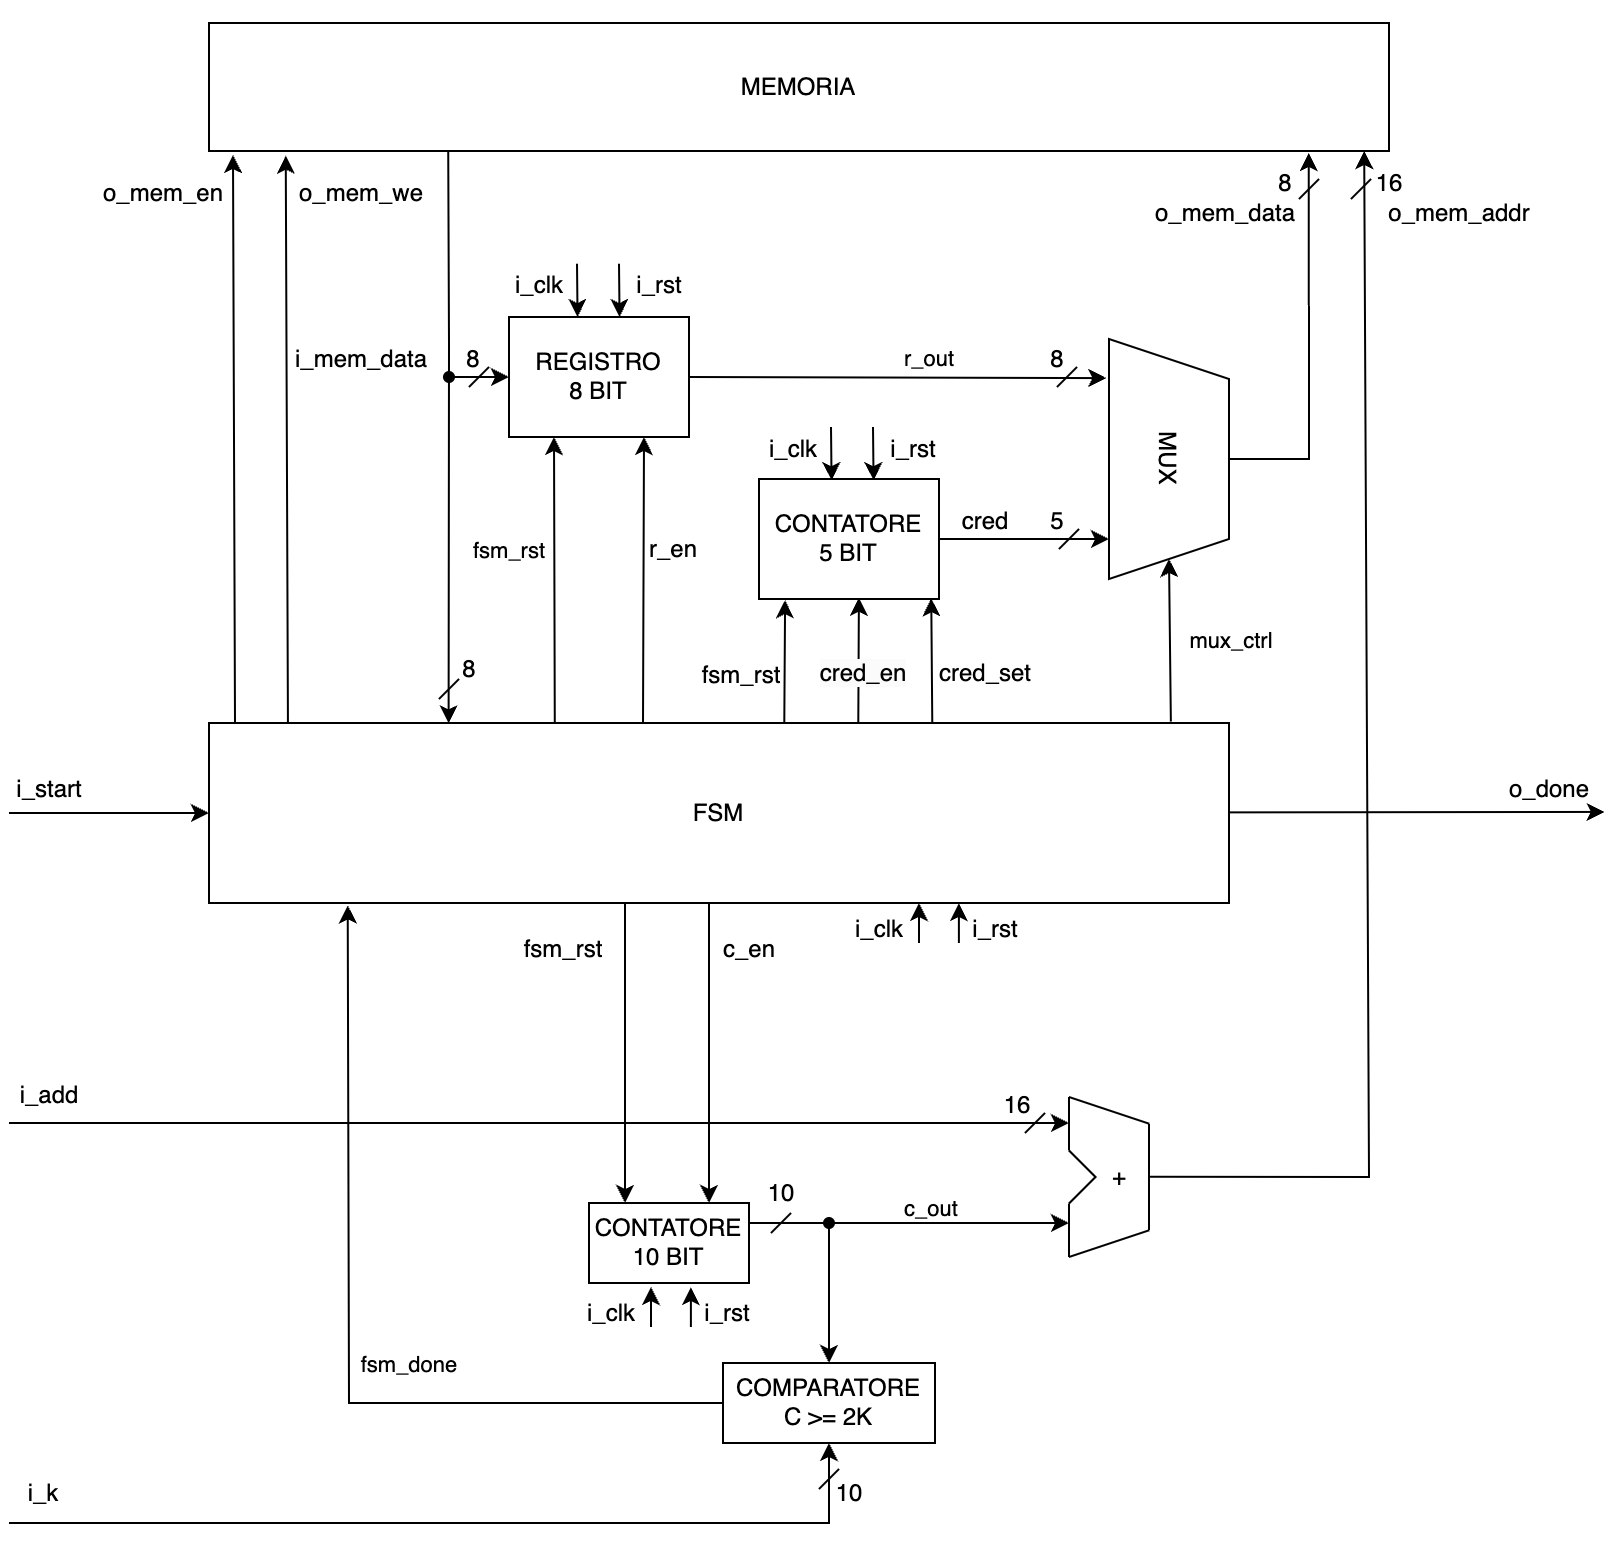
\includegraphics[width=1\textwidth]{figures/project.png}
    \caption{Rappresentazione strutturale del modulo}
    \label{fig:project}
\end{figure}

\subsection{Componenti}

\subsubsection{FSM}
\begin{figure}[H]
    \centering
    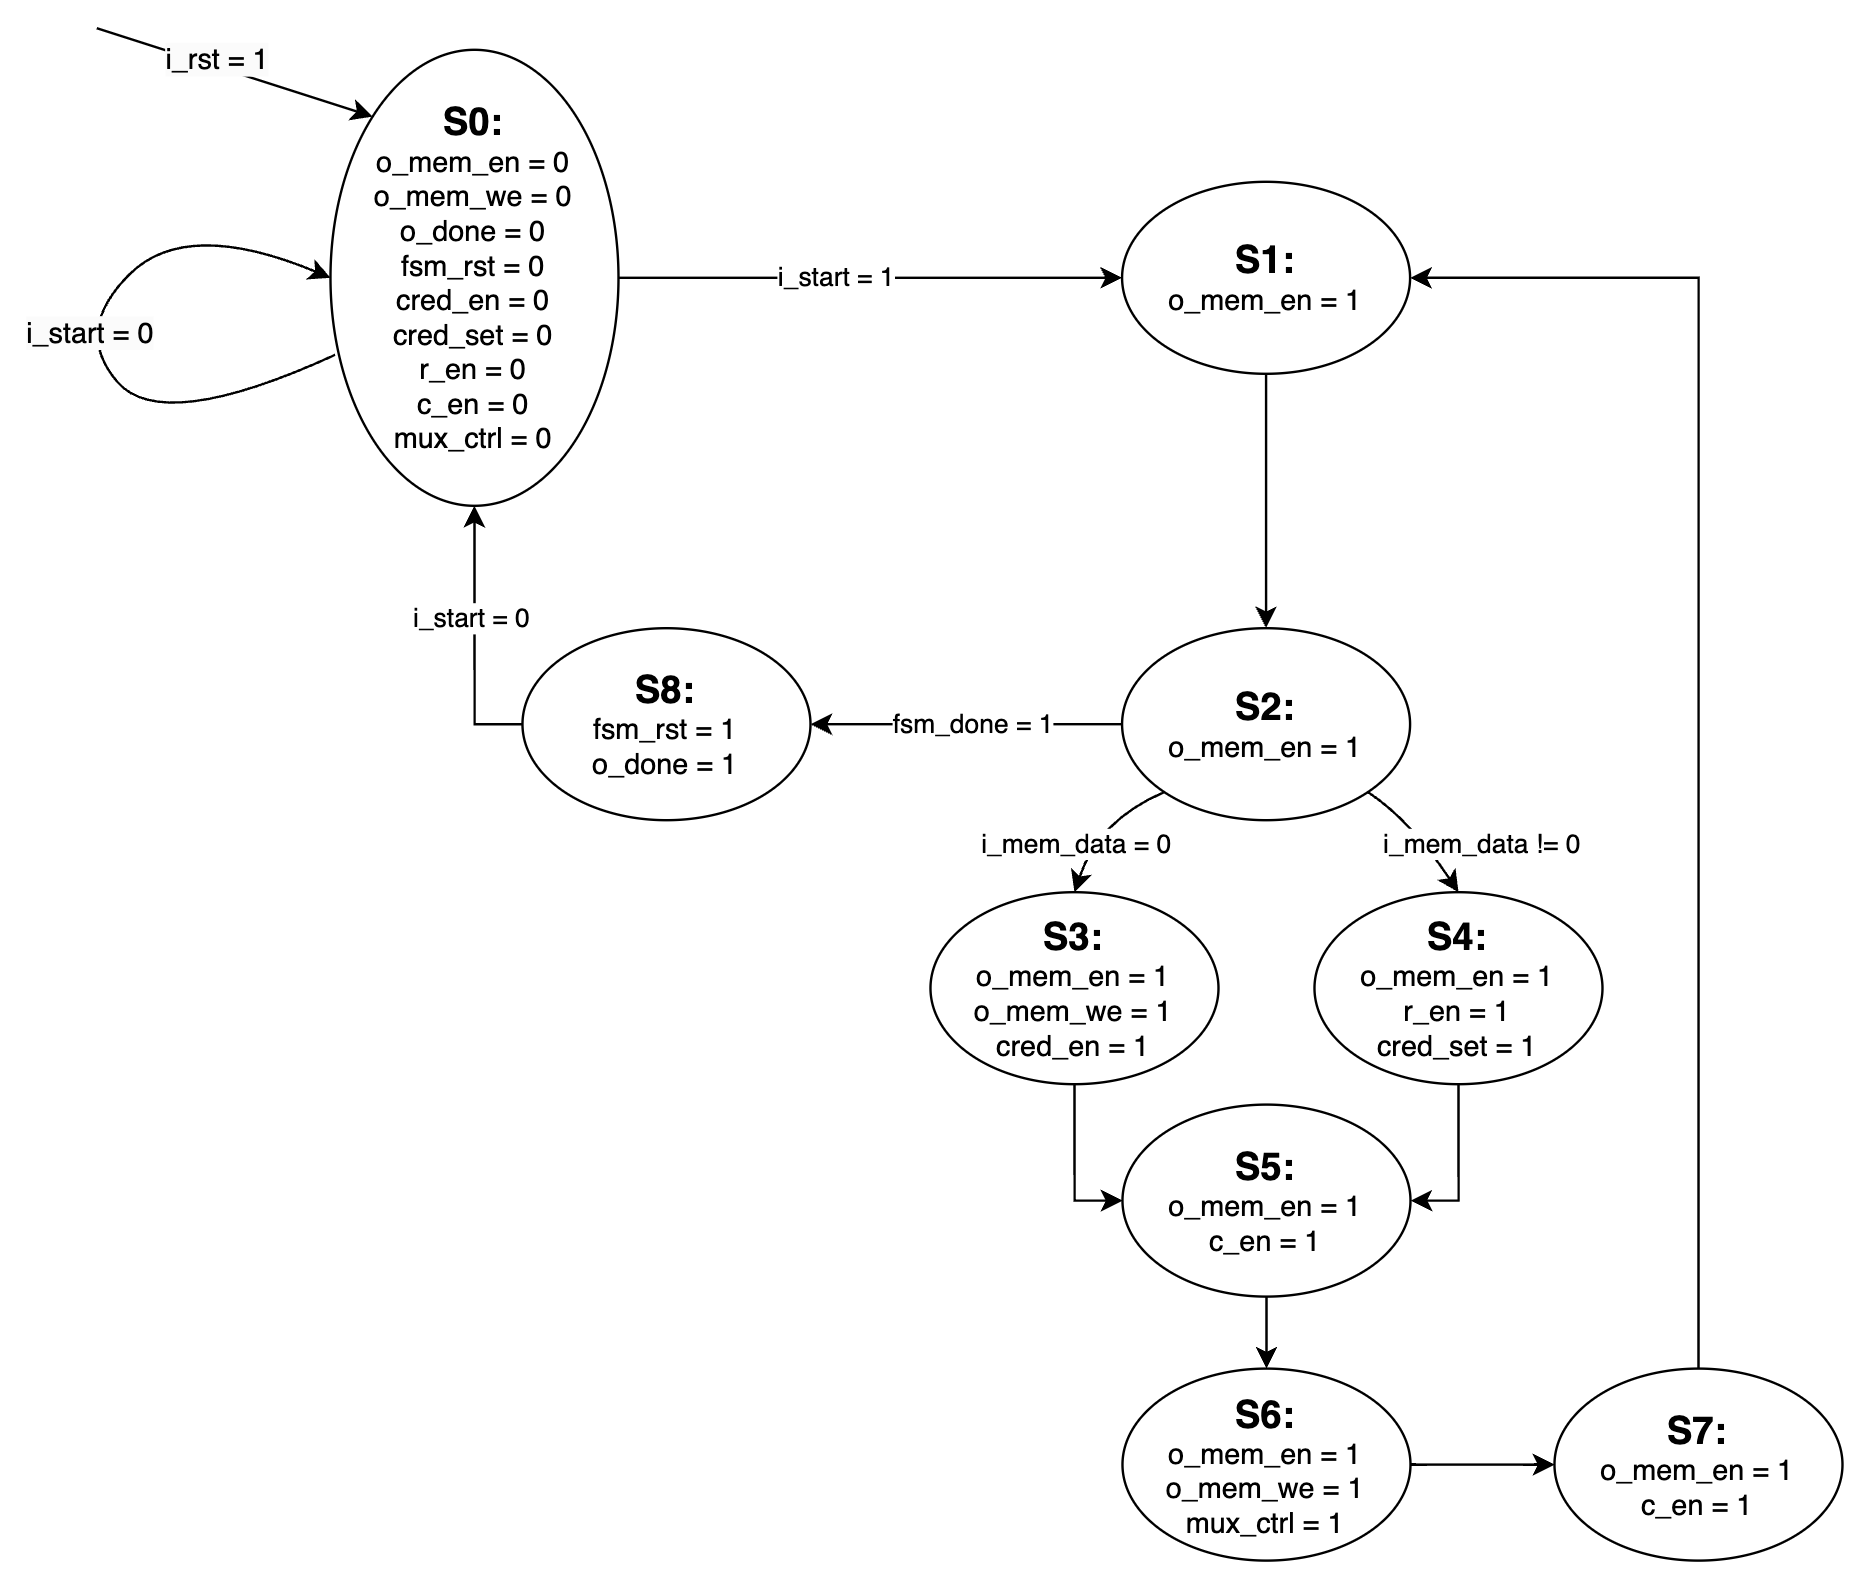
\includegraphics[width=1\textwidth]{figures/fsm.png}
    \caption{Diagramma degli stati}
    \label{fig:fsm}
\end{figure}

La FSM utilizzata è un esempio di macchina di Moore ed è quindi stata implementata con un process per il passaggio di stato ed uno per le uscite.
Essa (Figura \ref{fig:fsm}) è composta dai seguenti nove stati:

\begin{itemize}[itemsep=10pt]
	\item \texttt{\textbf{S0}}:\newline
	Stato iniziale di reset in cui si attende che venga alzato il segnale \lstinline[columns=fixed]{i_start}. In caso di segnale \lstinline[columns=fixed]{i_rst='1'} si torna in questo stato.
 	\item \texttt{\textbf{S1}}:\newline
	Stato in cui viene abilitata la lettura in memoria.
 	\item \texttt{\textbf{S2}}:\newline
	Stato in cui la FSM legge il dato e sceglie l'opportuna transizione:
        \begin{itemize}
        	\item \lstinline[columns=fixed]{i_mem_data = '0'} va in S3;
        	\item \lstinline[columns=fixed]{i_mem_data != '0'} va in S4;
        	\item \lstinline[columns=fixed]{fsm_done = '1'} va in S8.
        \end{itemize}
 	\item \texttt{\textbf{S3}}:\newline
	Stato in cui viene scritta la parola già presente nel registro in memoria e decrementata la credibilità.
 	\item \texttt{\textbf{S4}}:\newline
	Stato in cui viene memorizzata nel registro la nuova parola e inizializzata la credibilità.
 	\item \texttt{\textbf{S5}}:\newline
	Stato in cui ci si sposta al prossimo indirizzo in cui verrà salvata la credibilità.
 	\item \texttt{\textbf{S6}}:\newline
	Stato in cui viene scritta la credibilità
	\item \texttt{\textbf{S7}}:\newline
	Stato in cui ci si sposta al prossimo indirizzo per leggere la prossima parola.
 	\item \texttt{\textbf{S8}}:\newline
	Stato in cui si inizializzano i componenti e viene alzato il segnale di \lstinline[columns=fixed]{o_done}.
\end{itemize}

\newpage

\subsubsection{Contatore Credibilità}
\begin{figure}[H]
    \centering
    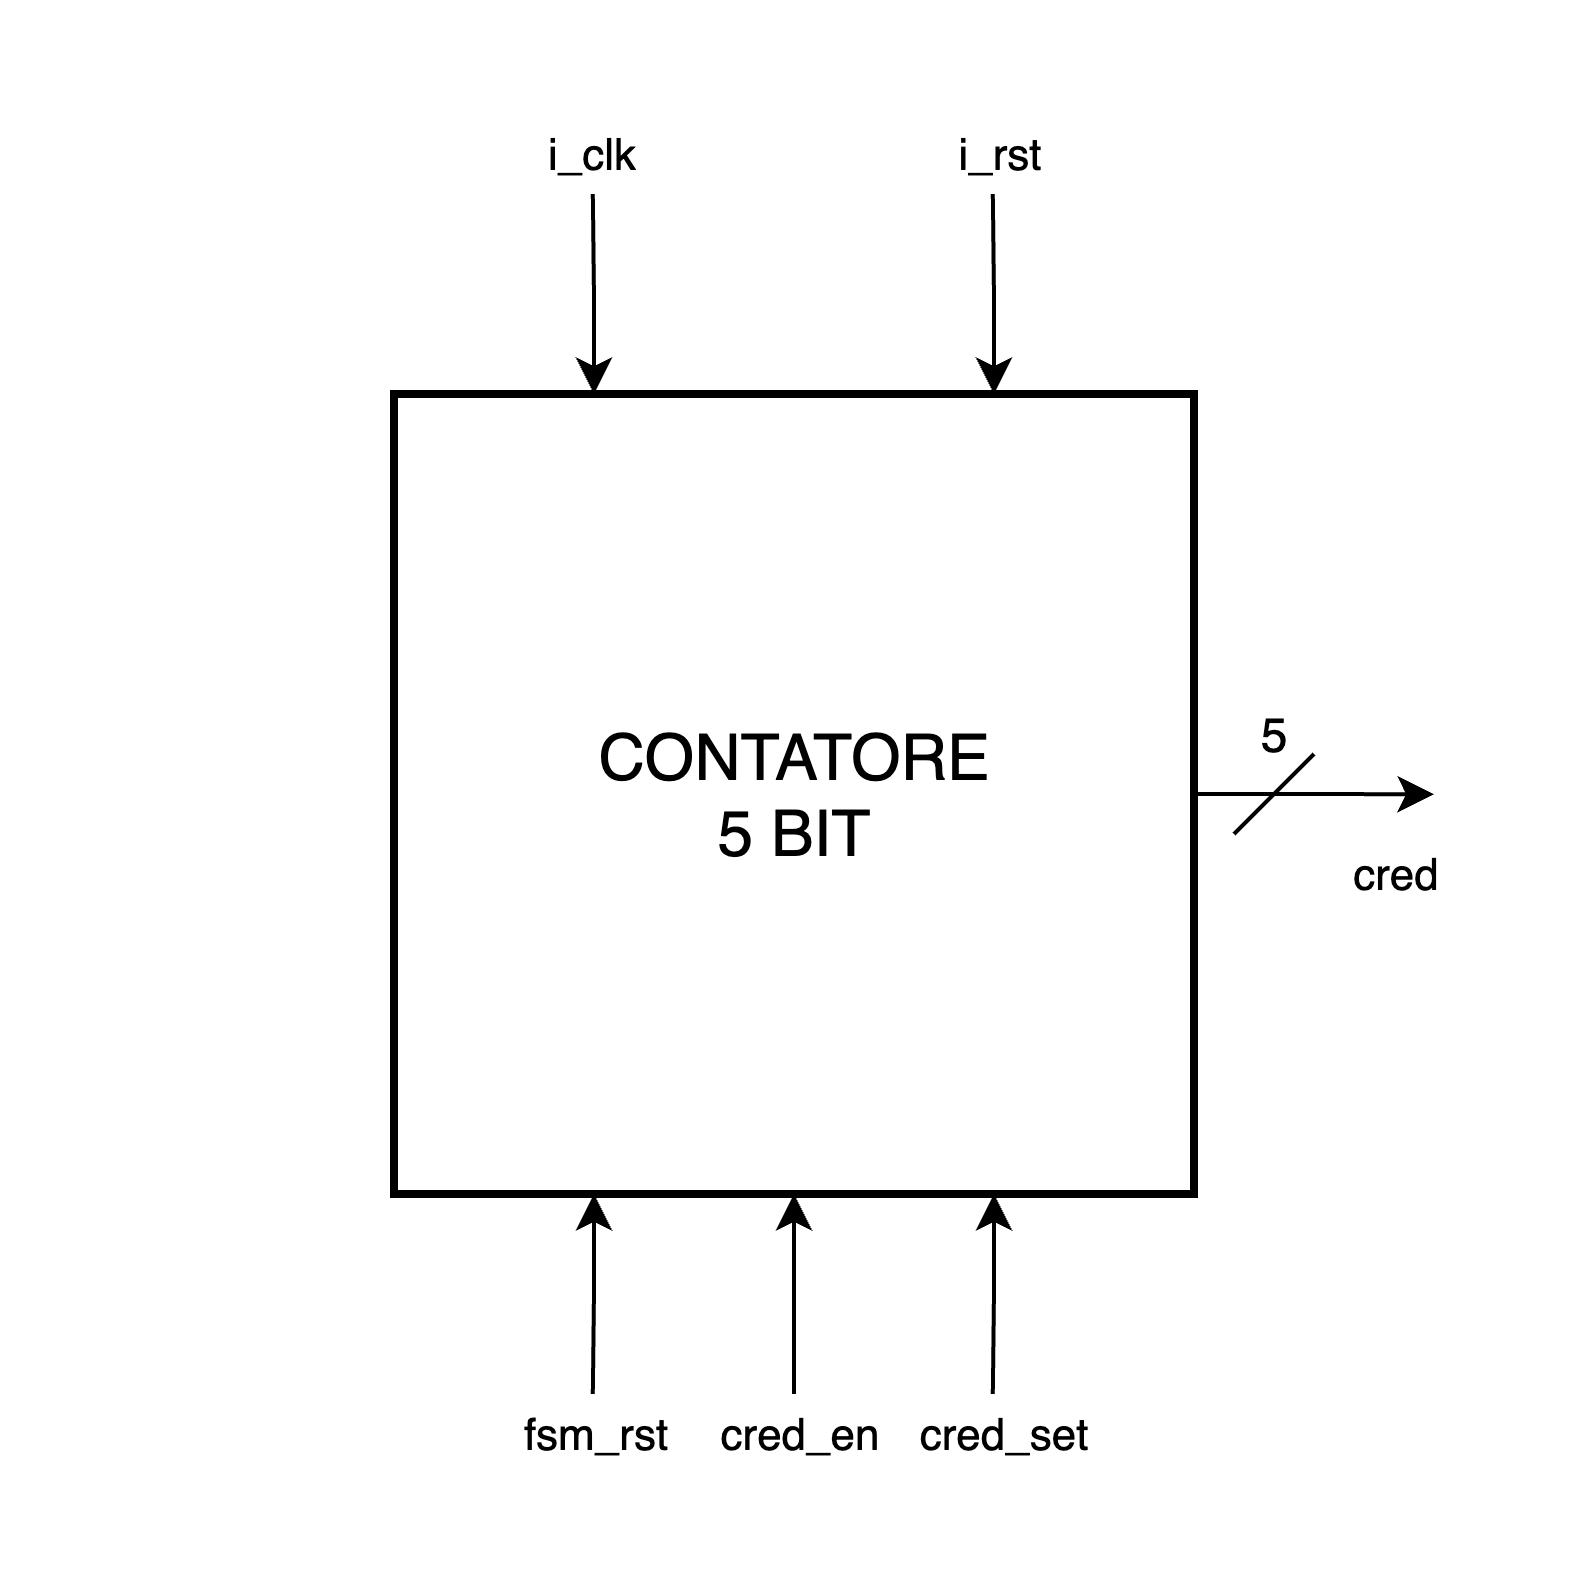
\includegraphics[width=0.4\textwidth]{figures/credibility.png}
    \caption{Rappresentazione della credibilità}
    \label{fig:credibility}
\end{figure}

Si occupa di tener conto della credibilità di una parola. A seguito del segnale di reset (sia esterno che dalla fsm) la credibilità è inizializzata a zero. Quando viene letta una parola valida viene ricevuto il segnale \lstinline[columns=fixed]{cred_set} che imposta la credibilità a 31. In caso di valore non specificato viene ricevuto il segnale \lstinline[columns=fixed]{cred_en} che permette di decrementare la credibilità.

\subsubsection{Multiplexer}
\begin{figure}[H]
    \centering
    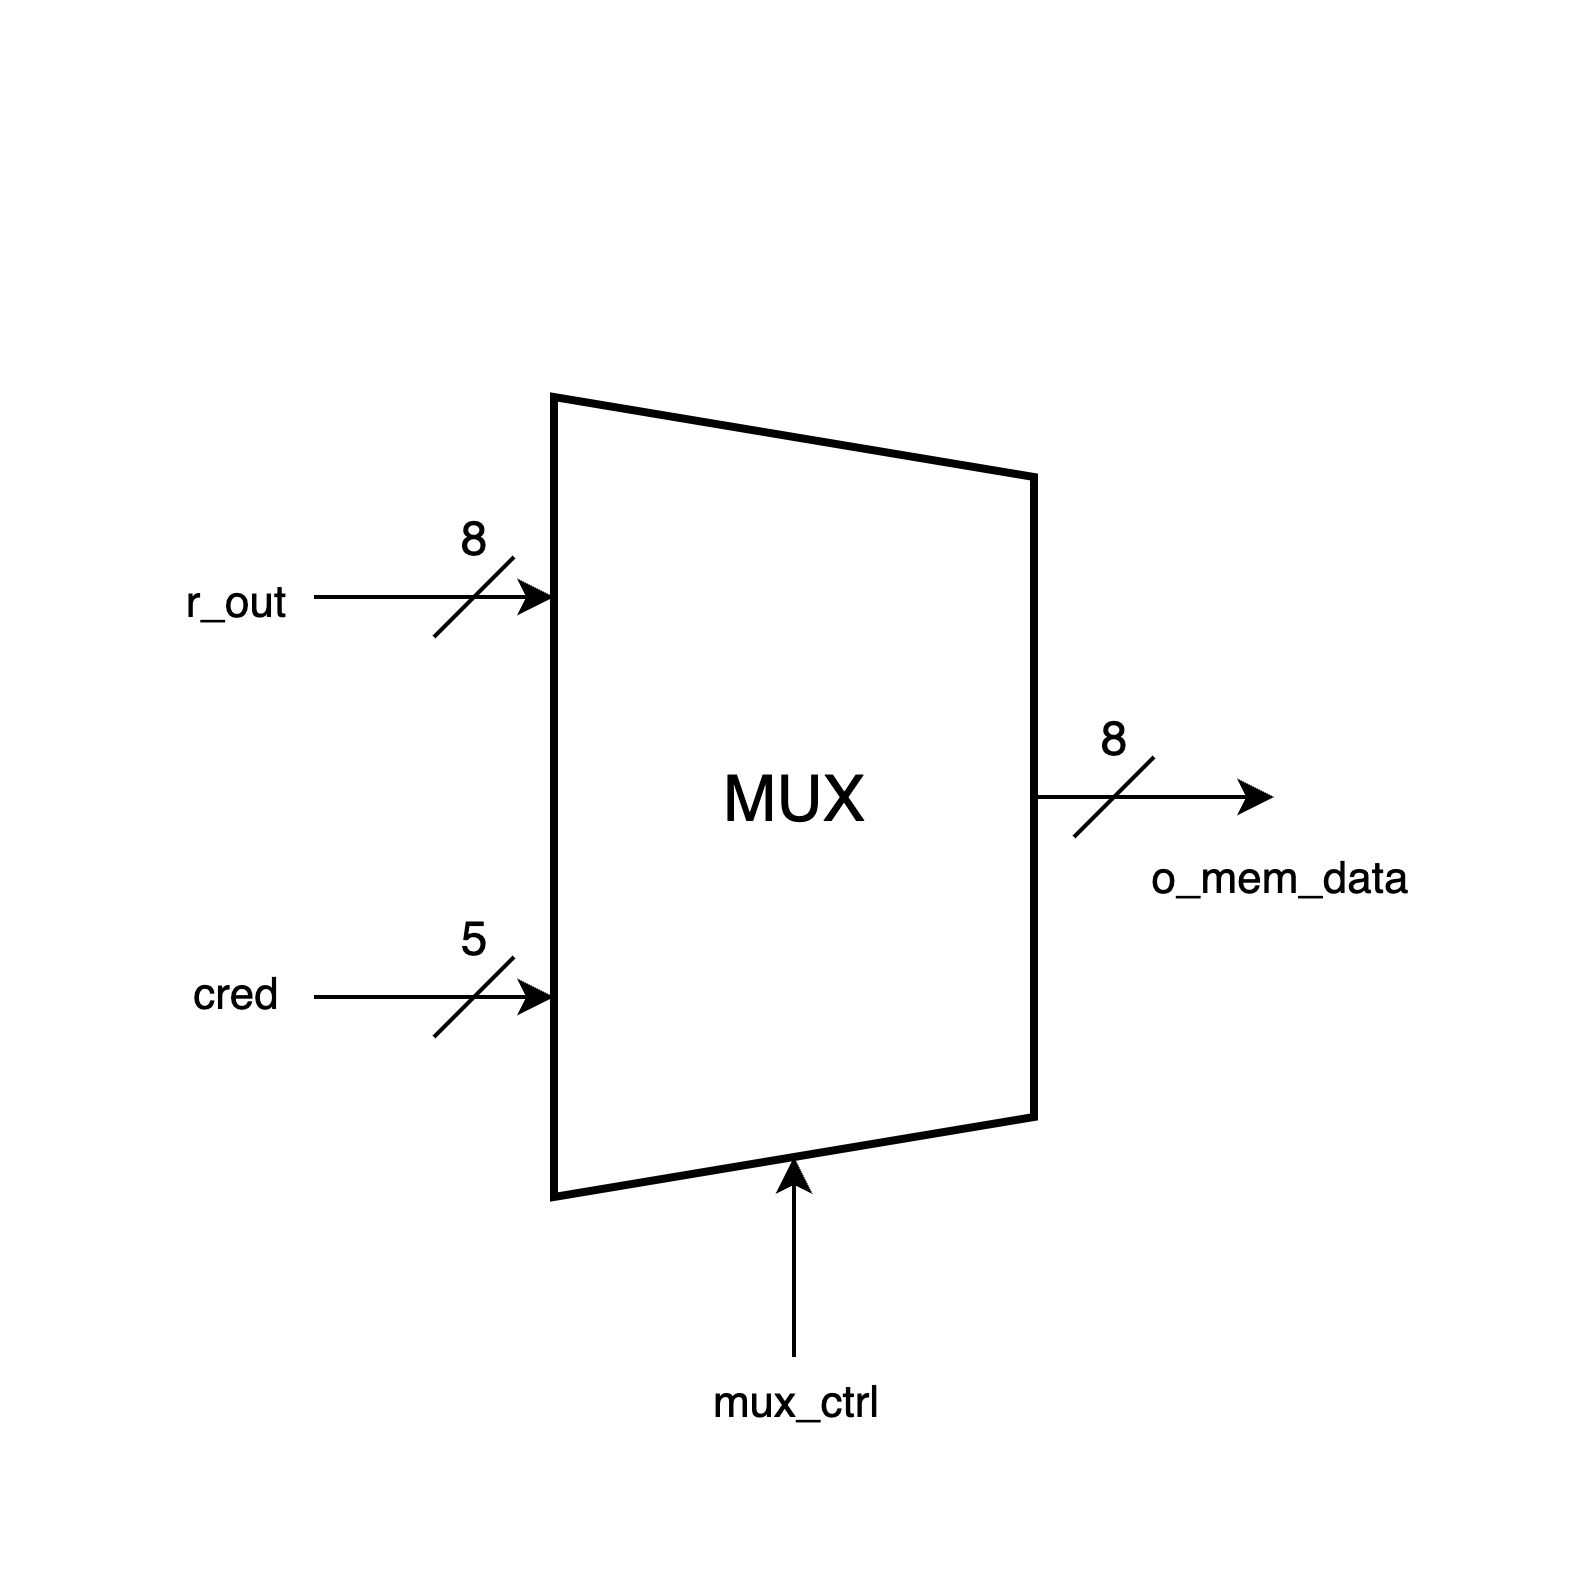
\includegraphics[width=0.4\textwidth]{figures/mux.png}
    \caption{Rappresentazione del multiplexer}
    \label{fig:mux}
\end{figure}

Si occupa di scegliere il dato da scrivere in memoria. Quando \lstinline[columns=fixed]{mux_ctrl = '0'} manderà la parola presente nel registro, quando  \lstinline[columns=fixed]{mux_ctrl = '1'} manderà la credibilità estesa ad 8 bit.

\subsubsection{Contatore Indirizzi}
\begin{figure}[H]
    \centering
    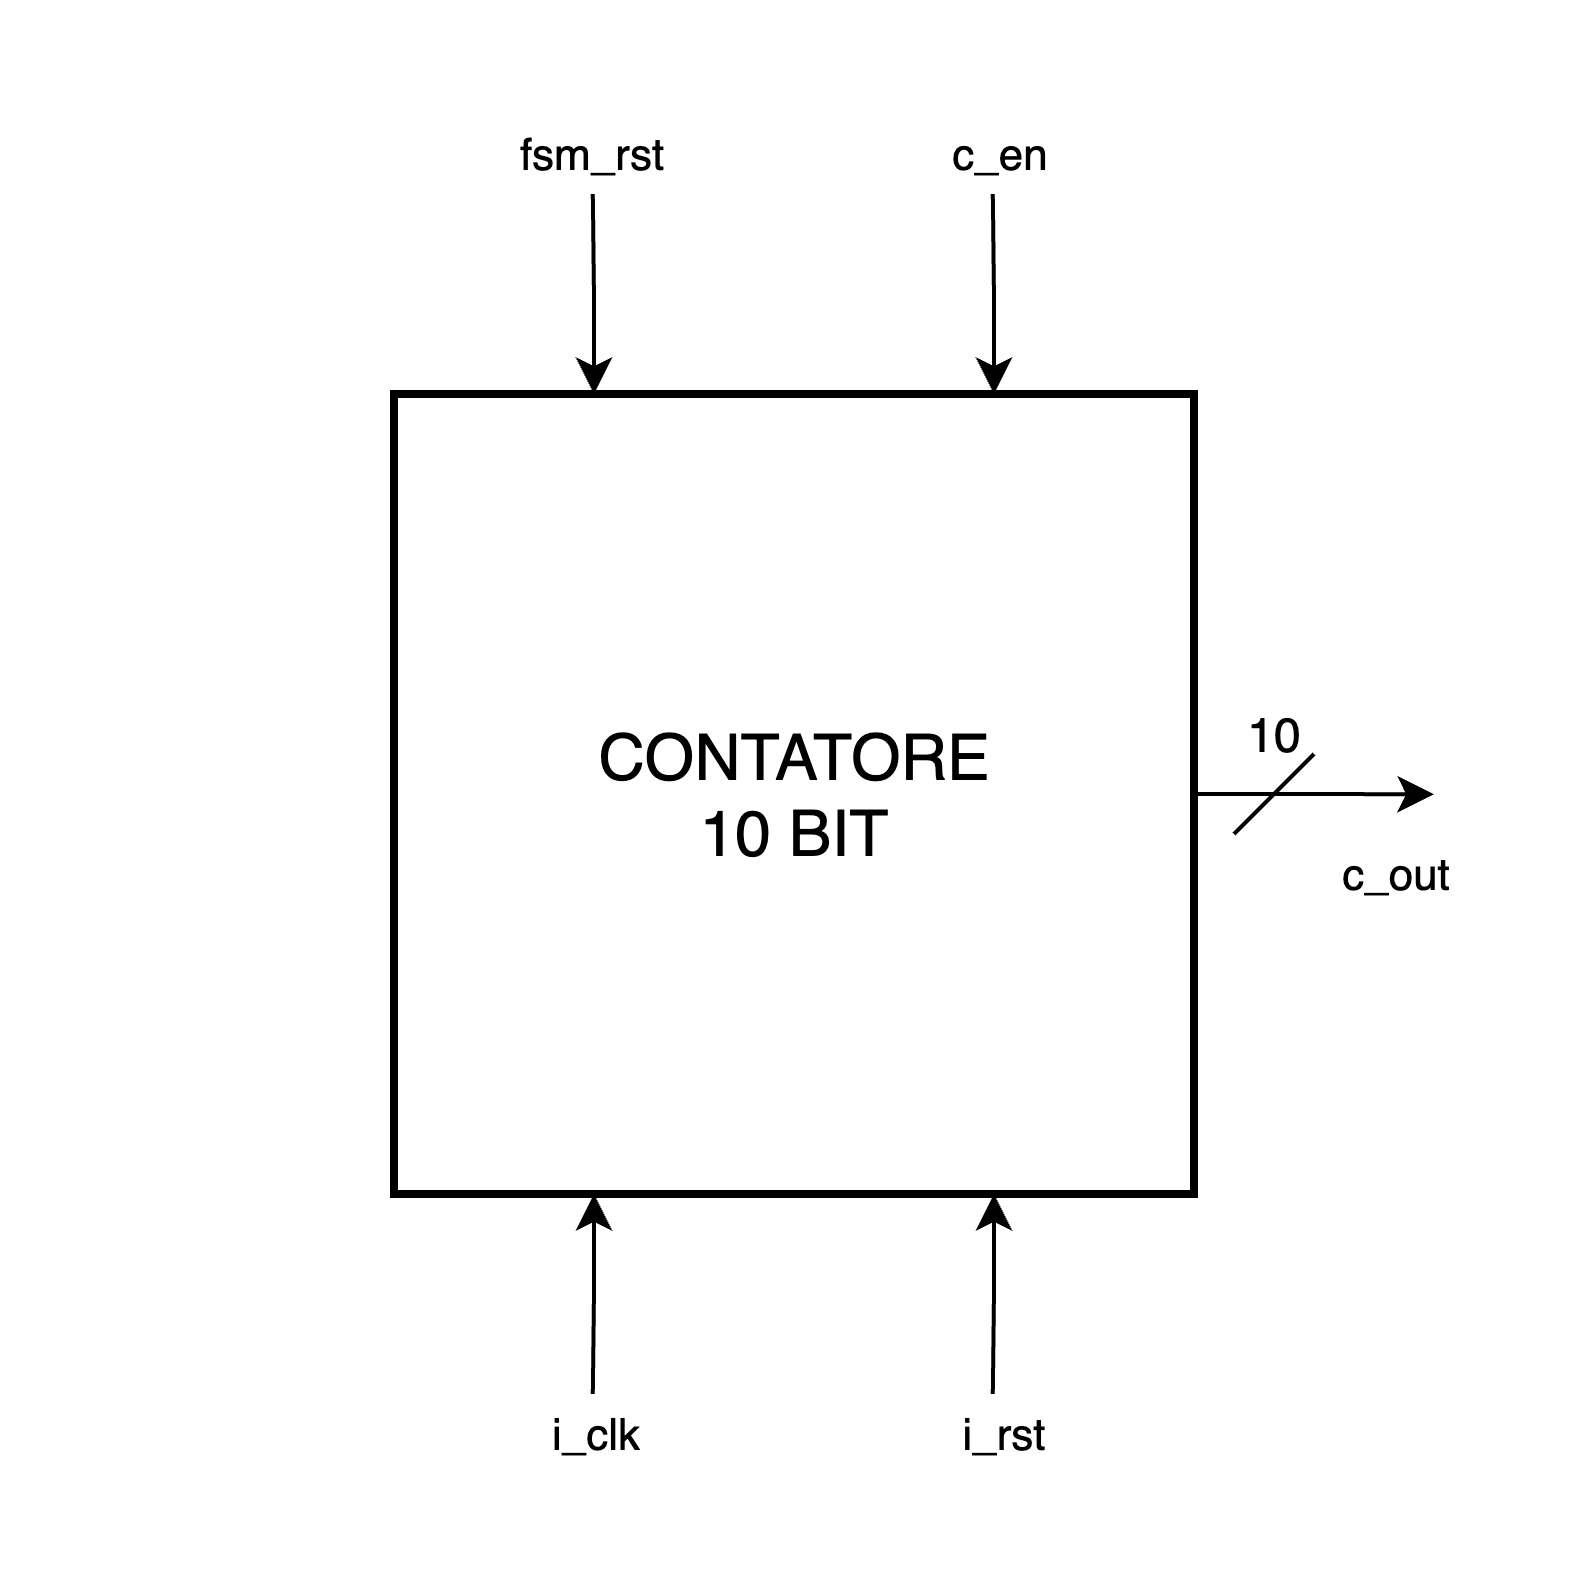
\includegraphics[width=0.4\textwidth]{figures/counter_10.png}
    \caption{Rappresentazione del contatore degli indirizzi}
    \label{fig:counter_10}
\end{figure}

Si occupa dell'avanzamento degli indirizzi di memoria. A seguito del segnale di reset (sia esterno che dalla fsm) il contatore è inizializzato a zero. Quando il segnale \lstinline[columns=fixed]{c_en} è alto permette al contatore di incrementare.

\subsubsection{Sommatore}
\begin{figure}[H]
    \centering
    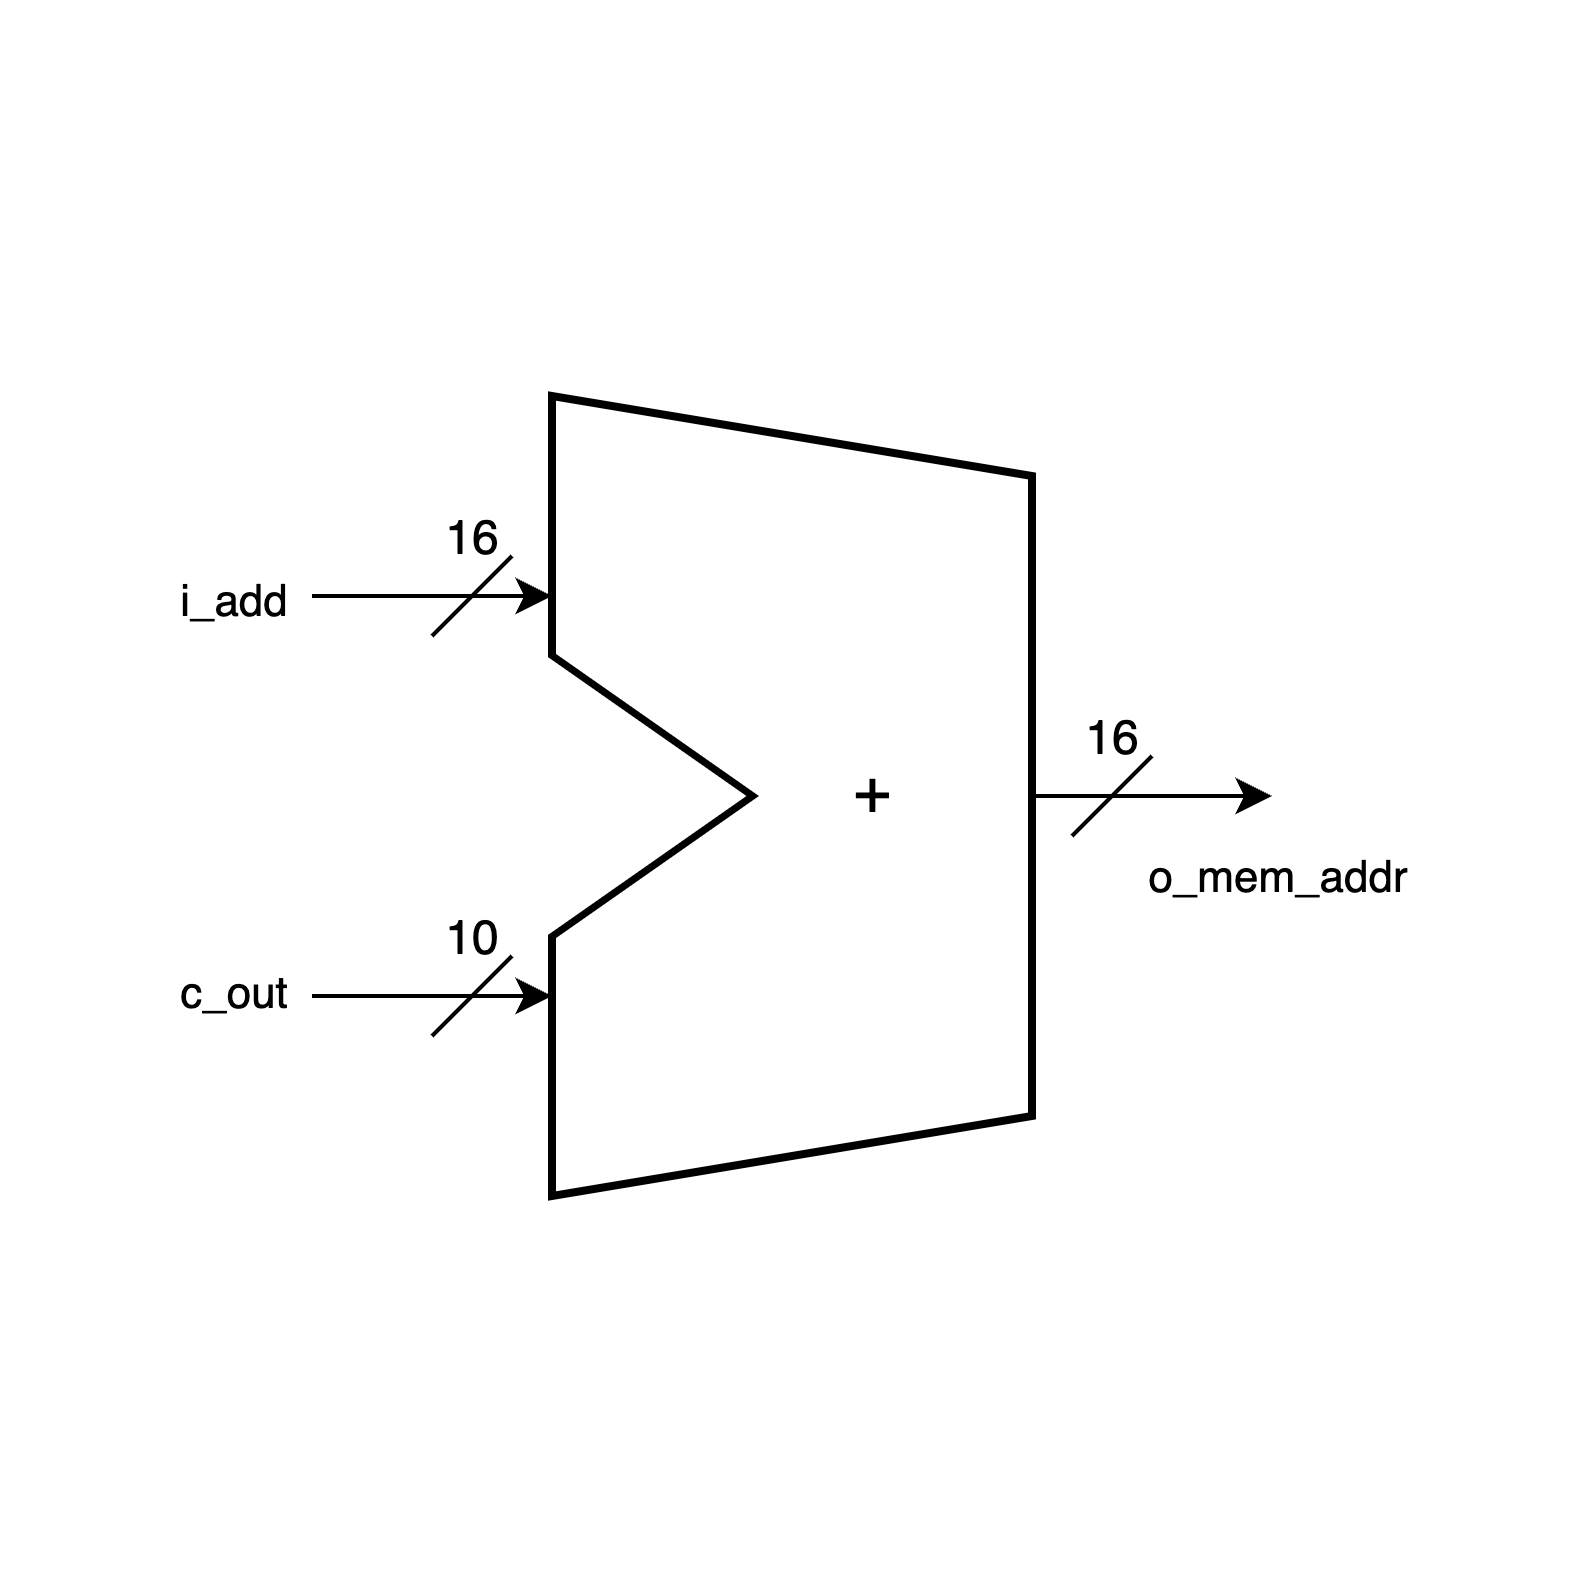
\includegraphics[width=0.4\textwidth]{figures/adder.png}
    \caption{Rappresentazione del sommatore}
    \label{fig:adder}
\end{figure}

Si occupa di trovare l'indirizzo di memoria su cui stiamo lavorando. Somma l'indirizzo di partenza e il contatore degli indirizzi.

\subsubsection{Comparatore}
\begin{figure}[H]
    \centering
    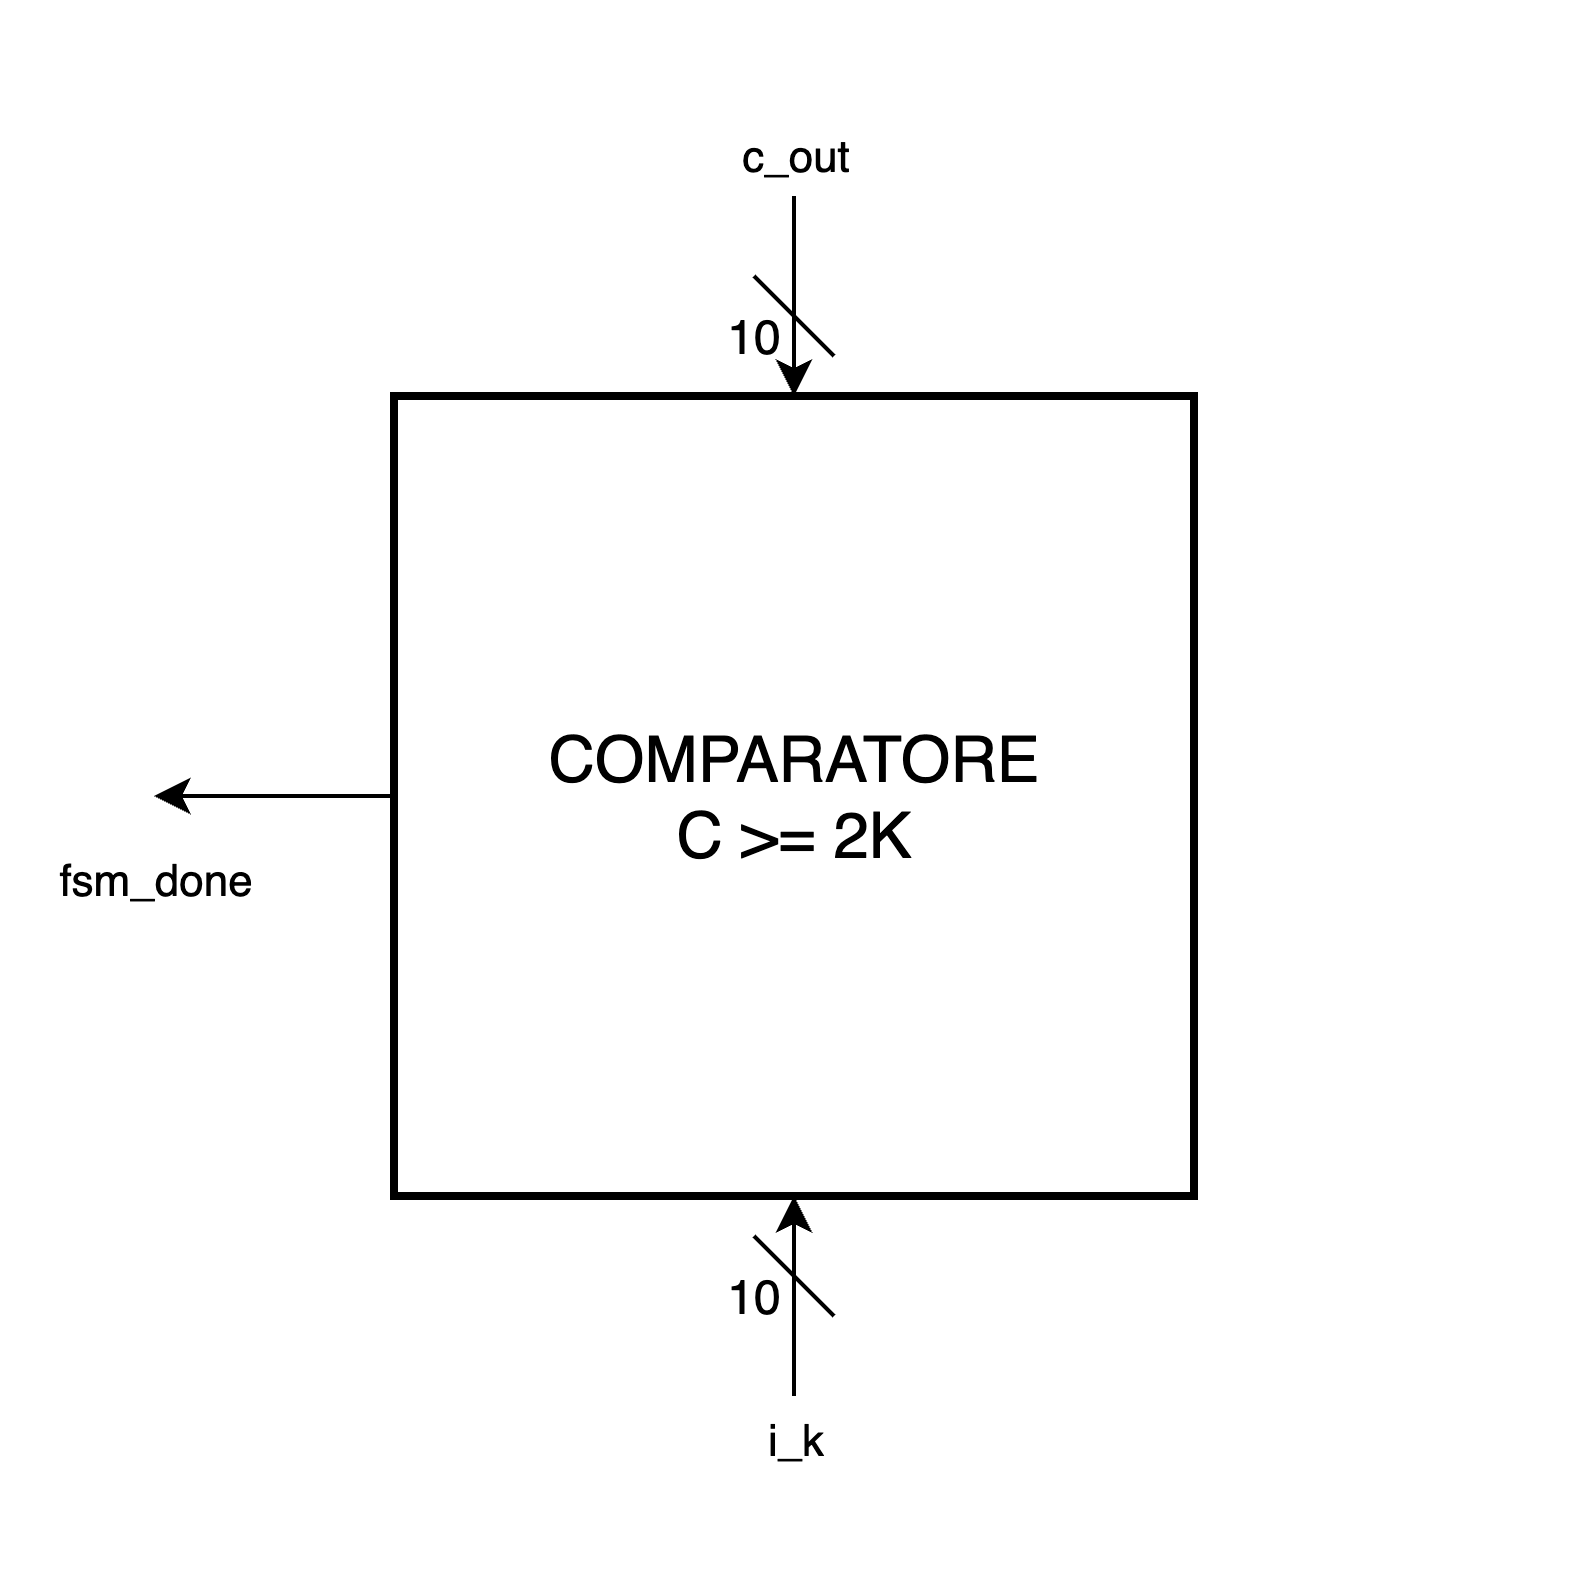
\includegraphics[width=0.4\textwidth]{figures/comparator.png}
    \caption{Rappresentazione del comparatore}
    \label{fig:comparator}
\end{figure}

Si occupa di notificare il termine della sequenza. Quando il contatore degli indirizzi raggiunge il valore 2K, dove K è il numero di parole della sequenza, il comparatore alza il segnale \lstinline[columns=fixed]{fsm_done}.

\subsubsection{Registro}
\begin{figure}[H]
    \centering
    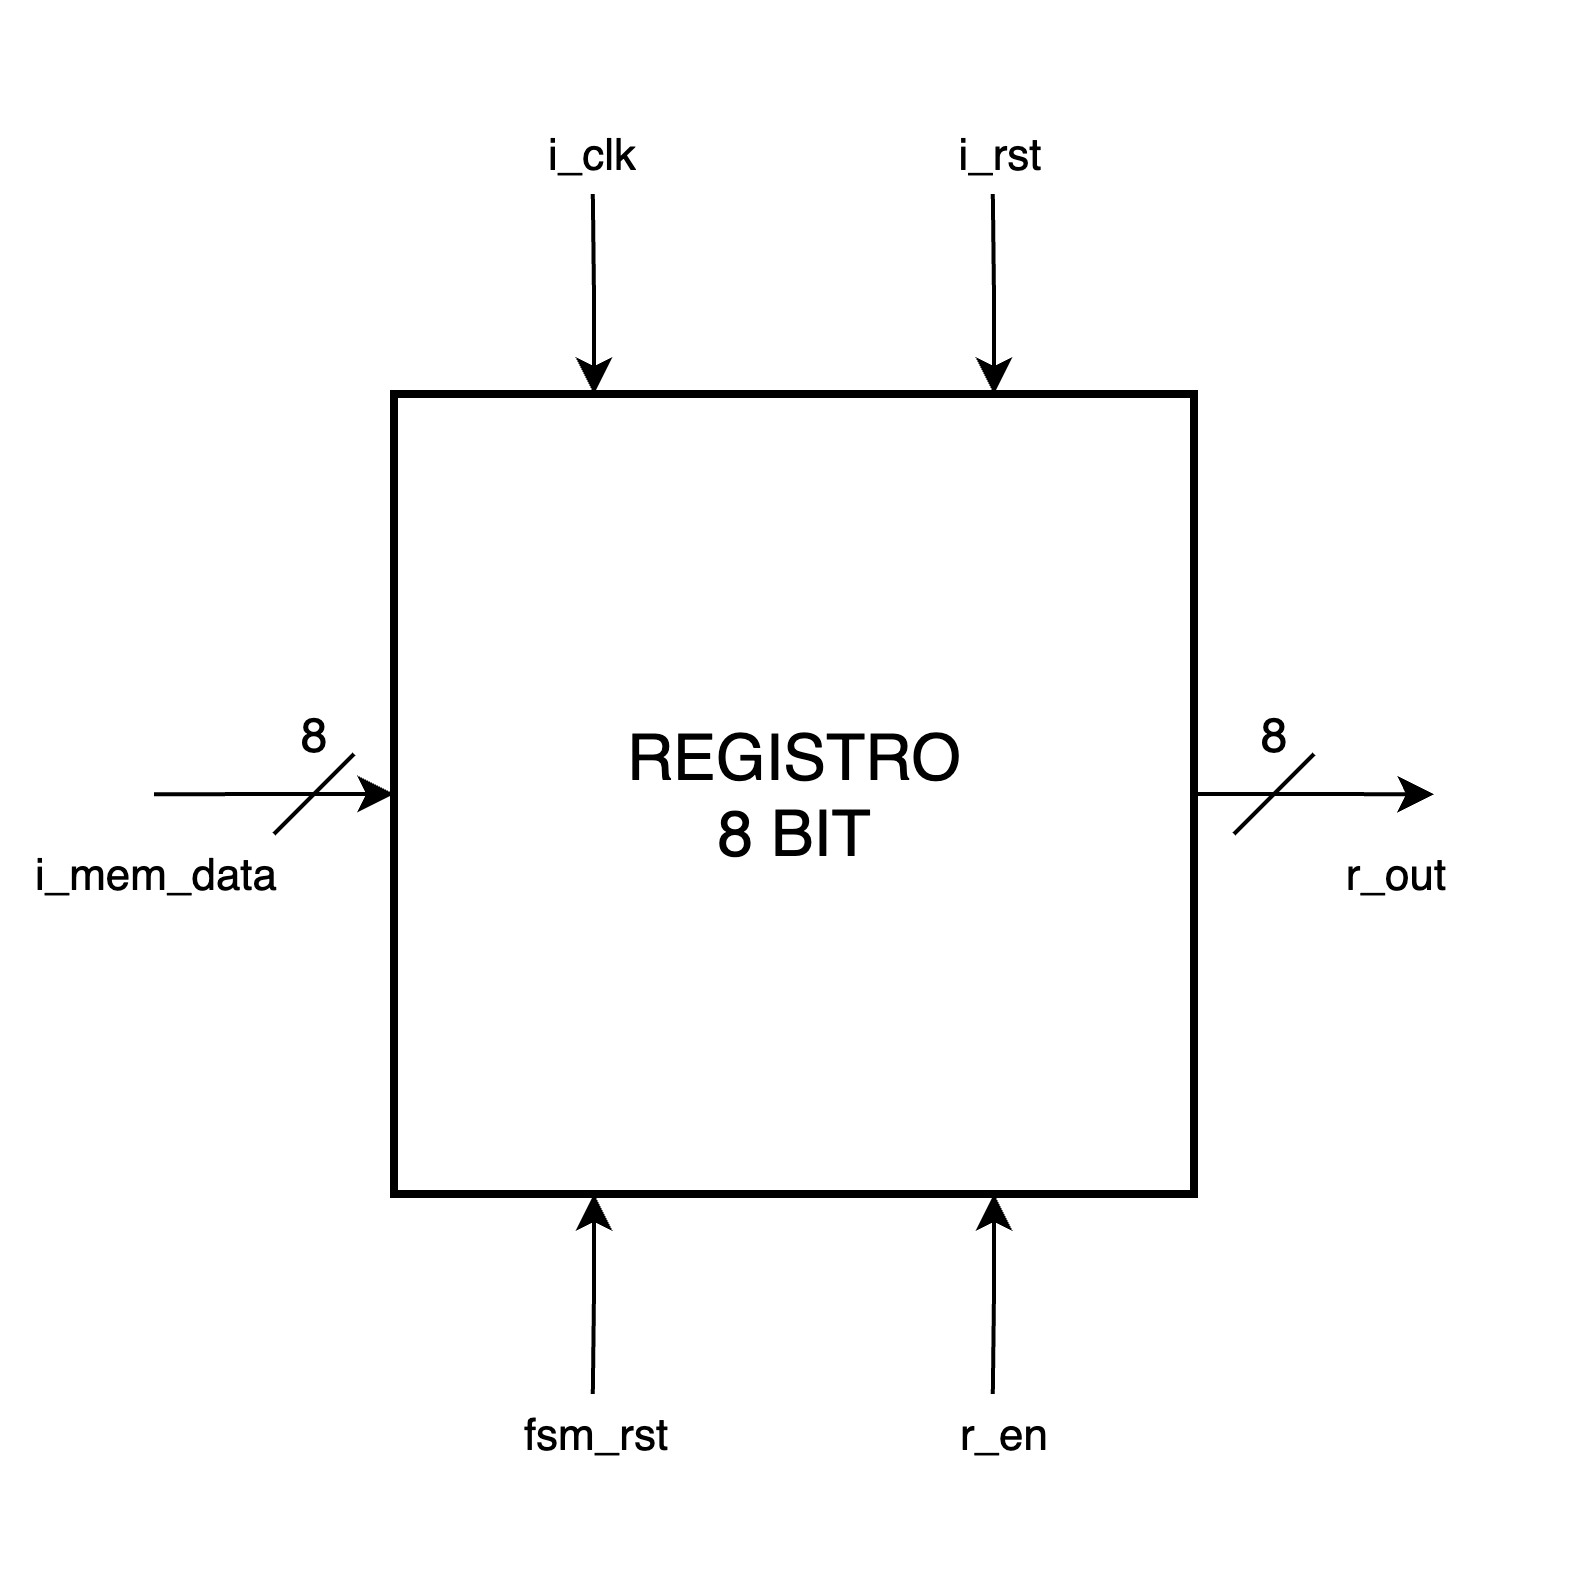
\includegraphics[width=0.4\textwidth]{figures/register_8.png}
    \caption{Rappresentazione del registro}
    \label{fig:register_8}
\end{figure}

Si occupa di salvare la parola valida che dovrà essere scritta in memoria in caso di valore non specificato. A seguito del segnale di reset (sia esterno che dalla fsm) il registro è inizializzato a zero. Quando il segnale di enable è alto il registro salva il valore di \lstinline[columns=fixed]{i_mem_data}.